% Use only LaTeX2e, calling the article.cls class and 12-point type.

\documentclass[12pt]{article}

% Users of the {thebibliography} environment or BibTeX should use the
% scicite.sty package, downloadable from *Science* at
% www.sciencemag.org/about/authors/prep/TeX_help/ .
% This package should properly format in-text
% reference calls and reference-list numbers.

\usepackage{scicite}

% Use times if you have the font installed; otherwise, comment out the
% following line.

\usepackage{times}
\usepackage{graphicx}
\usepackage{caption}
\usepackage{subcaption}
% The preamble here sets up a lot of new/revised commands and
% environments.  It's annoying, but please do *not* try to strip these
% out into a separate .sty file (which could lead to the loss of some
% information when we convert the file to other formats).  Instead, keep
% them in the preamble of your main LaTeX source file.


% The following parameters seem to provide a reasonable page setup.

\topmargin 0.0cm
\oddsidemargin 0.2cm
\textwidth 16cm 
\textheight 21cm
\footskip 1.0cm


%The next command sets up an environment for the abstract to your paper.

\newenvironment{sciabstract}{%
\begin{quote} \bf}
{\end{quote}}


% If your reference list includes text notes as well as references,
% include the following line; otherwise, comment it out.

\renewcommand\refname{References and Notes}

% The following lines set up an environment for the last note in the
% reference list, which commonly includes acknowledgments of funding,
% help, etc.  It's intended for users of BibTeX or the {thebibliography}
% environment.  Users who are hand-coding their references at the end
% using a list environment such as {enumerate} can simply add another
% item at the end, and it will be numbered automatically.

\newcounter{lastnote}
\newenvironment{scilastnote}{%
\setcounter{lastnote}{\value{enumiv}}%
\addtocounter{lastnote}{+1}%
\begin{list}%
{\arabic{lastnote}.}
{\setlength{\leftmargin}{.22in}}
{\setlength{\labelsep}{.5em}}}
{\end{list}}


% Include your paper's title here

\title{Copy Move Detection} 


% Place the author information here.  Please hand-code the contact
% information and notecalls; do *not* use \footnote commands.  Let the
% author contact information appear immediately below the author names
% as shown.  We would also prefer that you don't change the type-size
% settings shown here.

\author
{Anthony Sutardja, Kevin Tee\\
\\
\normalsize{Department of Computer Science}\\
\normalsize{University of California, Berkeley}\\
\normalsize{CS294-26 Final Project}\\
\\
\normalsize\texttt{\{anthonysutardja,kevintee\}@berkeley.edu} 
}

% Include the date command, but leave its argument blank.

\date{}



%%%%%%%%%%%%%%%%% END OF PREAMBLE %%%%%%%%%%%%%%%%



\begin{document} 

% Double-space the manuscript.

\baselineskip24pt
\setlength{\parskip}{1em}
\setlength{\parindent}{0em}
% Make the title.

\maketitle 



% Place your abstract within the special {sciabstract} environment.

\begin{sciabstract}
Abstract: ``Copy-move" forgery, in which a portion of the image is resampled to another region, is a common photo manipulation technique used to alter picture content. Previous work in detecting this type of forgery has shown inaccurate results and inefficient processing time. We propose a combination of methods that results in fast and more accurate copy-move detection performance. Our method finds invariant features within the image and looks for matches using a modified version of nearest neighbors on oriented patches of the images. Potential corresponding matches are filtered by whether they fit into a set of transformations given by RANSAC.
\end{sciabstract}

% In setting up this template for *Science* papers, we've used both
% the \section* command and the \paragraph* command for topical
% divisions.  Which you use will of course depend on the type of paper
% you're writing.  Review Articles tend to have displayed headings, for
% which \section* is more appropriate; Research Articles, when they have
% formal topical divisions at all, tend to signal them with bold text
% that runs into the paragraph, for which \paragraph* is the right
% choice.  Either way, use the asterisk (*) modifier, as shown, to
% suppress numbering.

\section*{Introduction}
Photo manipulation tools have been becoming more powerful and accessible to use than ever before. Almost anyone can open up their favorite photo manipulation tool, like Adobe PhotoShop, and change the image to enhance and alter it. As these techniques get more and more advanced, the distinction between what is real and what is been crafted is becoming harder to distinguish, which means that the human eye has difficulty interpreting which images are authentic.

In this paper, we examine the detection of a particular type of image forgery known as copy-move forgery. Copy-move forgery is when portions of the image are resampled to another part of the image with the intent to change the photo's meaning and context. An example of such an attack is replacing a portion of the image with more buildings as seen in Figure 1 [2].

There are many existing methods that attempt to detect copy-move forgery. However, some of these methods have large processing times of up to 2600 seconds (around 45 minutes) [1] and other methods do not achieve reliable detections [7].

We explore a combination of methods that yield reliable copy-move detections in a reasonable amount of time.


\begin{figure}
\centering
\begin{subfigure}{.5\textwidth}
  \centering
  \includegraphics[width=.8\linewidth]{../images/extension.png}
  \caption{Original image}
  \label{fig:sub1}
\end{subfigure}%
\begin{subfigure}{.5\textwidth}
  \centering
  \includegraphics[width=.8\linewidth]{../images/extension_copy.png}
  \caption{Copy-moved image}
  \label{fig:sub2}
\end{subfigure}
\caption{An example comparison of a copy move forgery where a portion of the image has been replaced with buildings sampled from the same image.}
\label{fig:test}
\end{figure}


\section*{Methodology}
Our method draws inspiration from a technique for stitching photos into into a panorama [6]. We follow a large portion of the panorama stitching pipeline in that we detect interest points, create oriented descriptors around the interest points, find potential matches, and estimate the transformation from the source to destination. Instead of applying this method to image stitching, we use this technique for identifying key features that have a strong correlation to other portions of the image. This is analogous to ``stitching" the photo in question to itself.

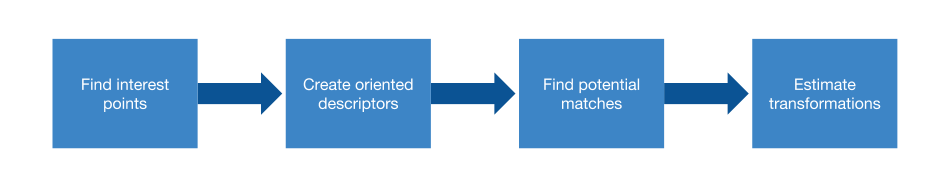
\includegraphics[width=1.0\linewidth]{./gfx/cm_pipeline.png}

\subsection*{Interest points}
To get interest points, we found the Harris corners, or points that have a high gradient in both the x and y direction within a 3x3 window [6]. We then use one of two methods to select a subset of the Harris corners: Adaptive Non-Maximal Suppression (ANMS) or corner-based sorting. 

The reason for filtering interest points is for speed. Filtering the points for a subset is necessary to drastically decrease running time. Although using every interest point found can lead to very accurate detections, comparing every interest point is computationally expensive and leads to extremely high processing times [1]. Furthermore, the filtering is also helpful for reducing the number of iterations that RANSAC needs to estimate the various copy-move transformations.

The two different interest point filtering methods both have significantly different use cases.

\begin{figure}
\centering
\begin{subfigure}{.5\textwidth}
  \centering
  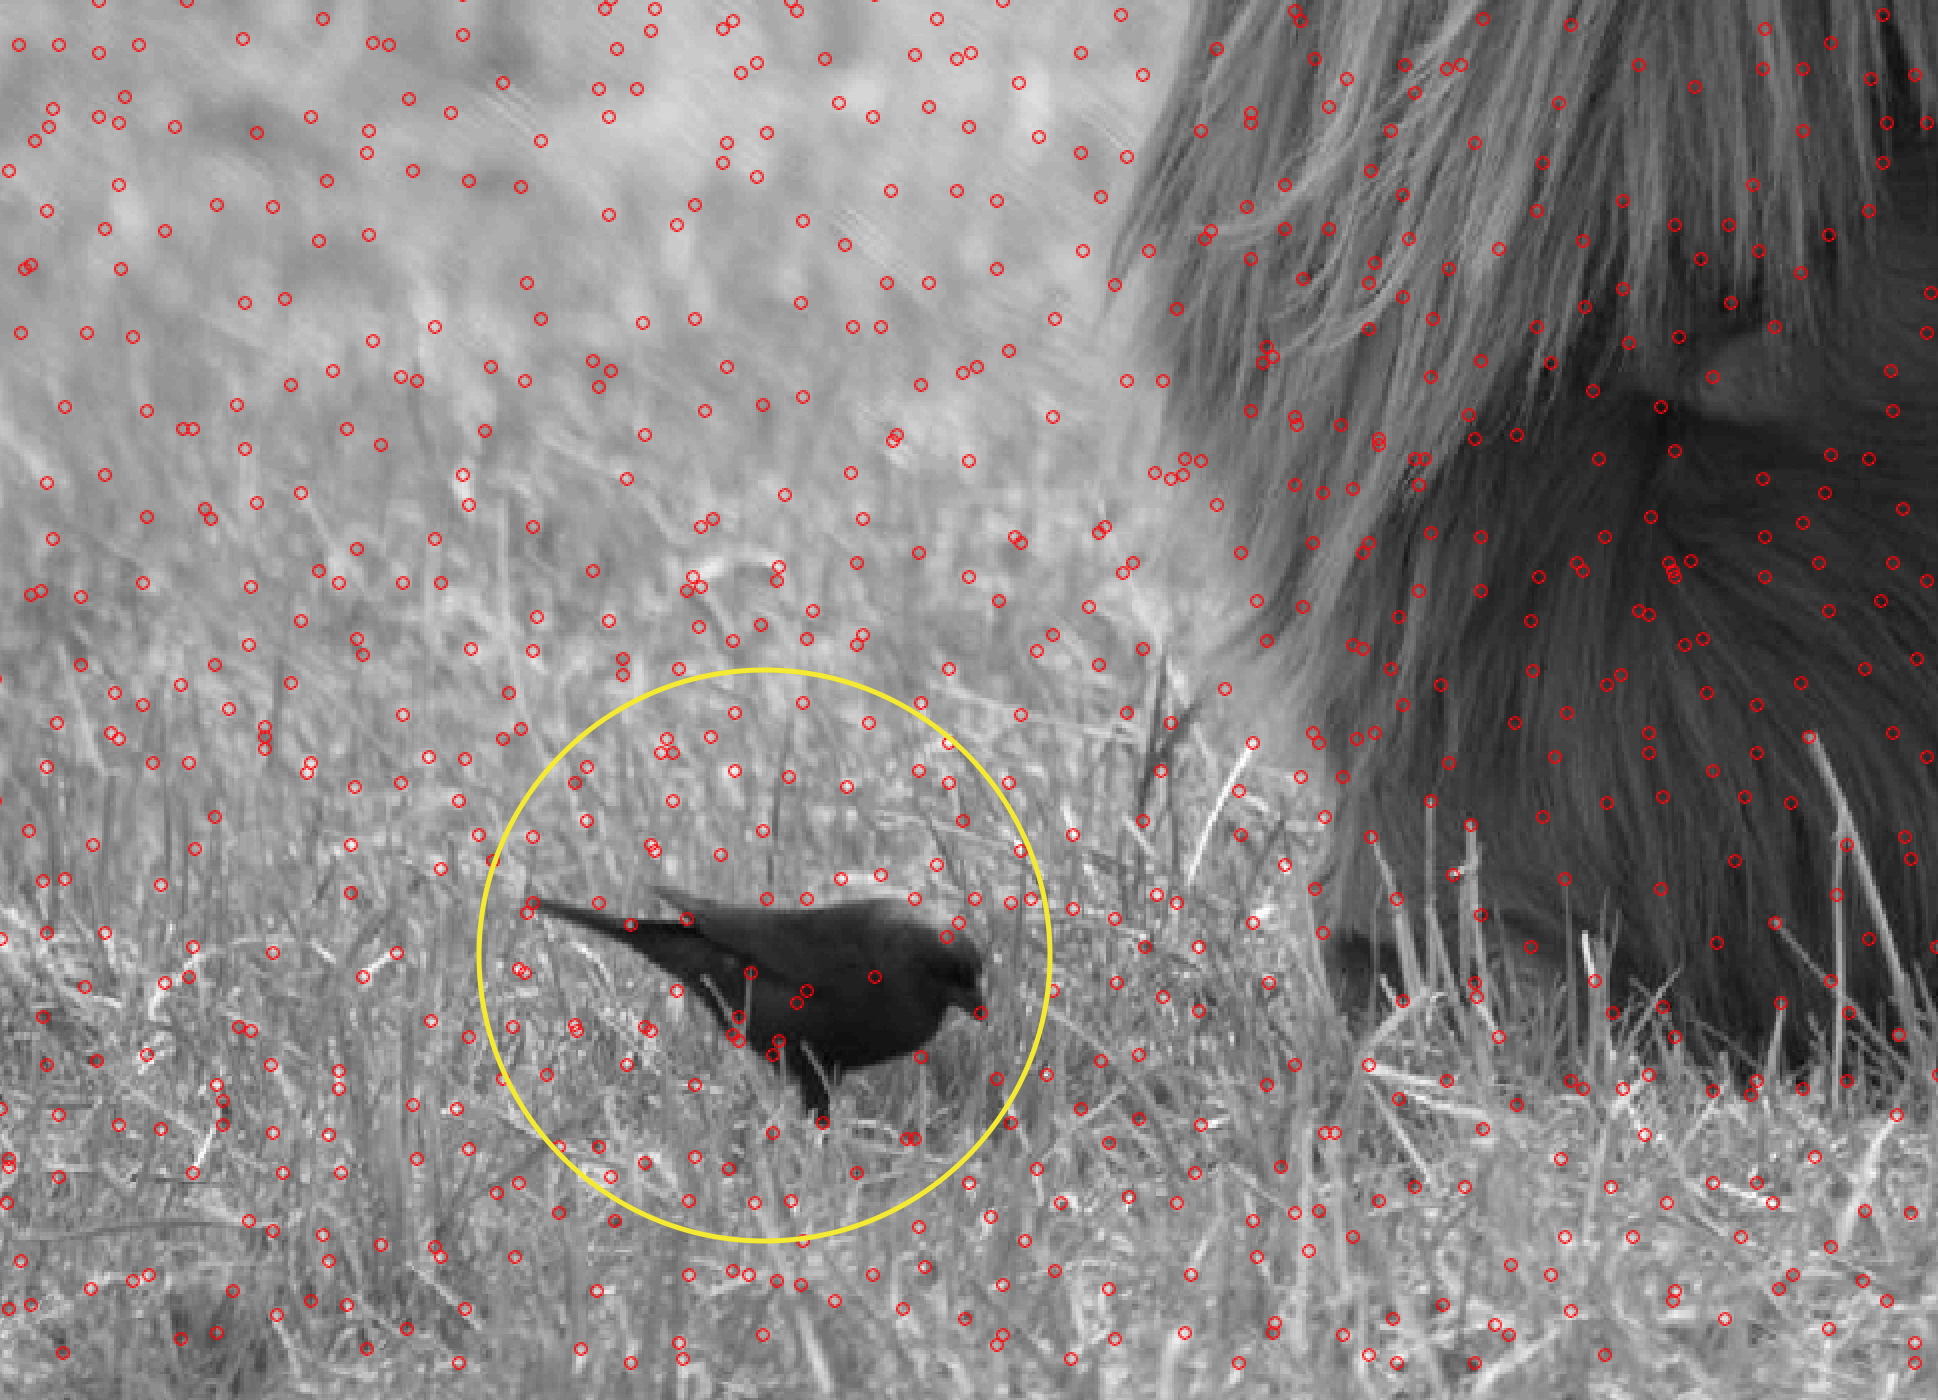
\includegraphics[width=.8\linewidth]{./gfx/ip_bird_anms.png}
  \caption{Interest points from ANMS}
  \label{fig:sub1}
\end{subfigure}%
\begin{subfigure}{.5\textwidth}
  \centering
  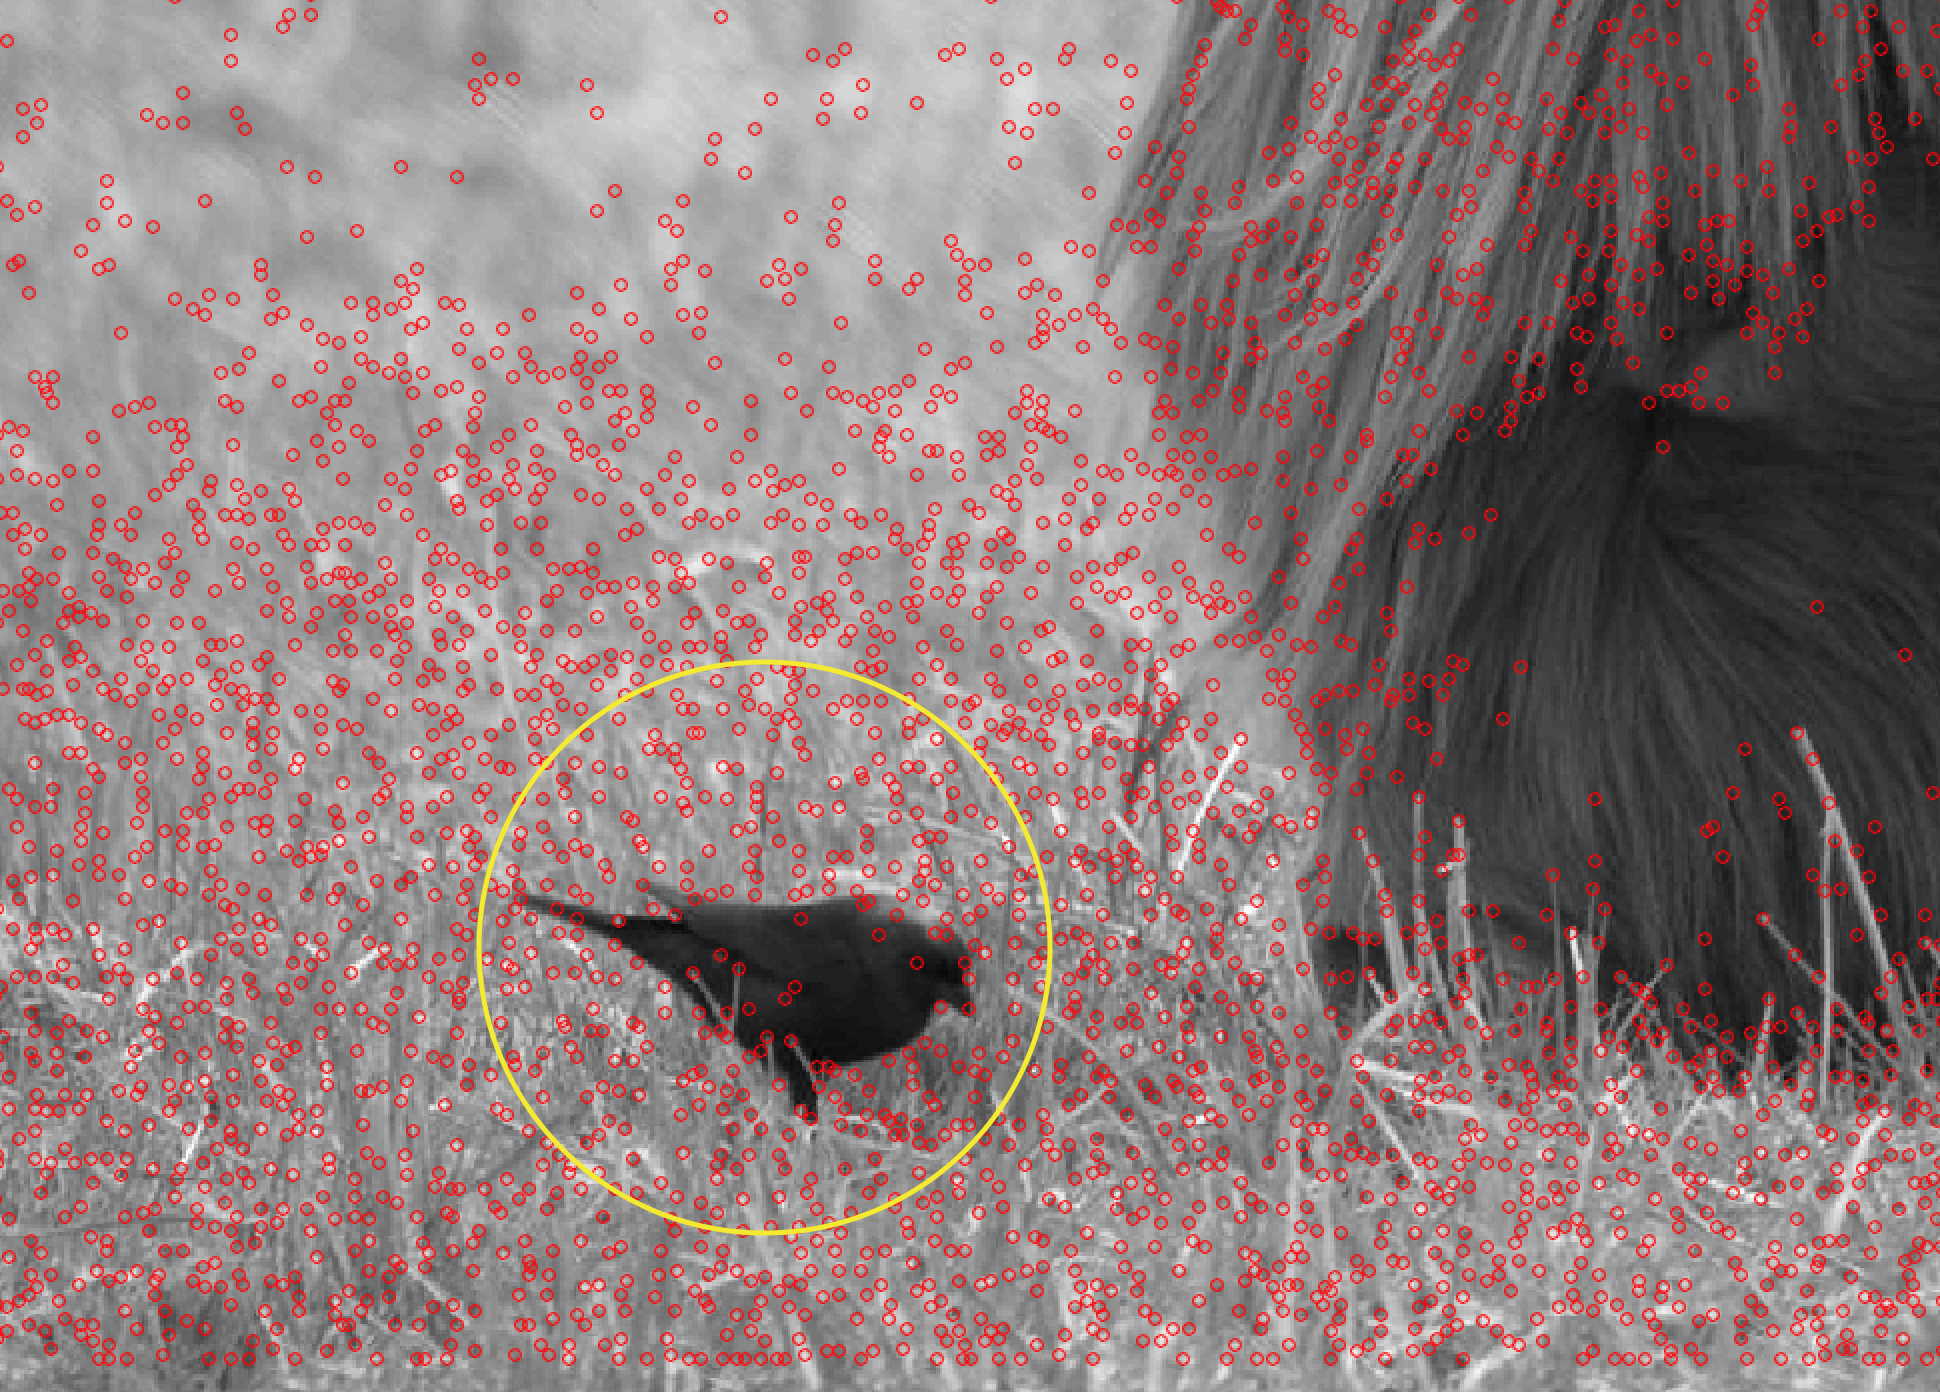
\includegraphics[width=.8\linewidth]{./gfx/ip_bird_high.png}
  \caption{Interest points from corner-based sorting}
  \label{fig:sub2}
\end{subfigure}
\begin{subfigure}{.5\textwidth}
  \centering
  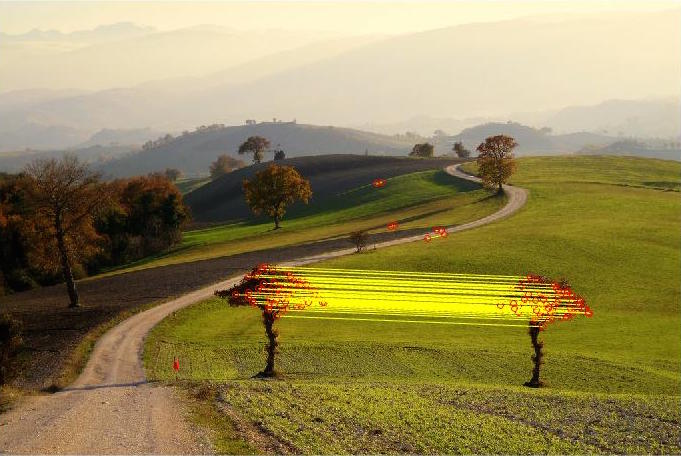
\includegraphics[width=.8\linewidth]{./gfx/ip_high.jpg}
  \caption{Detection with top harris corners}
  \label{fig:sub1}
\end{subfigure}%
\begin{subfigure}{.5\textwidth}
  \centering
  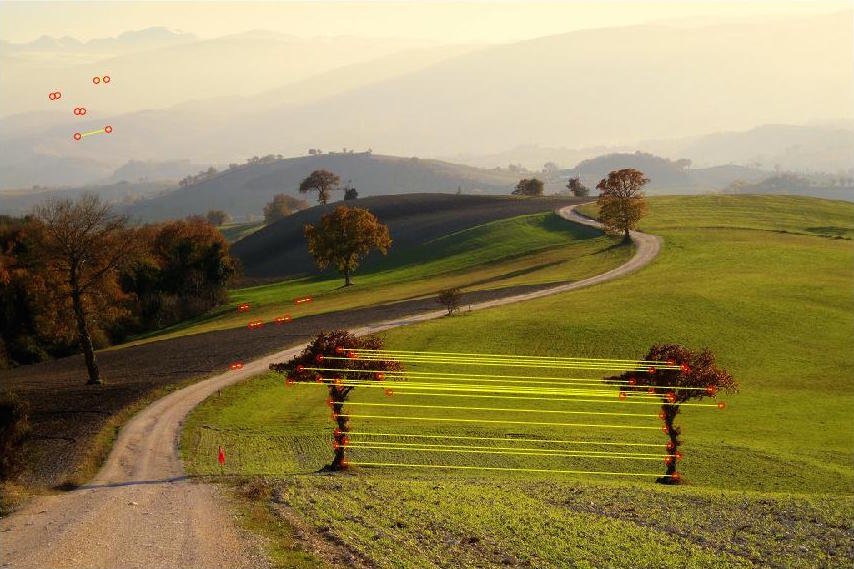
\includegraphics[width=.8\linewidth]{./gfx/ip_anms.jpg}
  \caption{Detection with ANMS}
  \label{fig:sub2}
\end{subfigure}
\caption{Figure 2(a) and 2(b) shows the contrast between using ANMS vs corner based sorting on small regions of manipulation; the bird has been copied and corner based sorting is able to capture more interest points for matching. Figure 2(c) and 2(d) show the difference between the locality of detection from corner-based sorting and the spread of detection from ANMS.}
\label{fig:test}
\end{figure}

In corner-based sorting, we take the Harris corners that have the highest Harris corner value, regardless of their distance to other points. Taking the top $N$ interest points from corner-based sorting helps capture more localized details. This is especially important with images that have extremely small manipulations, since copy-move transformation estimation requires at least a few points in order to come up with an accurate transformation.

In ANMS, we take Harris corners that are high in value and spread relative. This methodology is directly taken from the MOPS paper; please see the paper for more details on its implementation [6]. Using ANMS helps detection of a broader region of copy-move instances since the collection of interest points are more spread out. This is useful in capturing the full context of the copy-moved manipulation.

\subsection*{Descriptors}
We experimented with two different descriptors, the box descriptor and scale invariant feature transform (SIFT) descriptor.

For the box descriptor, we first implemented a naive box descriptor that did not take orientation into account. The box descriptor is created by sampling a 40x40 window that is Gaussian blurred (at $\sigma = 1.0$) and then downsampled to an 8 x 8 window, which is subsequently rescaled such that the features are zero mean unit variance. This descriptor worked well in identifying strictly translational copy move instances, but was a poor descriptor for rotated copy-move instances.

In order to make our box descriptor rotationally invariant, we oriented the windows such that the dominant gradient direction was aligend with the axis of each Gaussian blurred 40x40 window (with $\sigma = 4.0$). The dominant gradient was found by bucketing each pixel's orientation into ten 36 degree bucket. Each entry into the bucket was  was weighted by the gaussian coefficient based on each pixel's distance to the central interest point and the magnitude of each pixel's gradient. The weighted average of all the point orientations that were placed into the largest bucket was used to then calculate the overall weighted orientation of the descriptor. We also included the weighted orientation of buckets that were local maximas (taking the buckets that were at least $0.8$ times largest peak). This technique worked very well in identifying rotational copy-move as seen in Figure 3.

\begin{figure}
\centering
\begin{subfigure}{.5\textwidth}
  \centering
  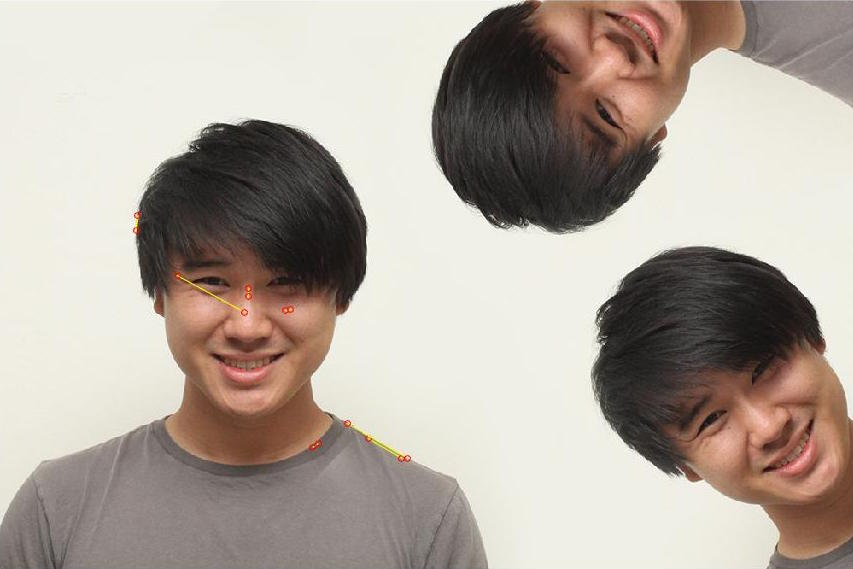
\includegraphics[width=.8\linewidth]{./gfx/without_rotation.jpg}
  \caption{Without oriented box descriptors}
  \label{fig:sub1}
\end{subfigure}%
\begin{subfigure}{.5\textwidth}
  \centering
  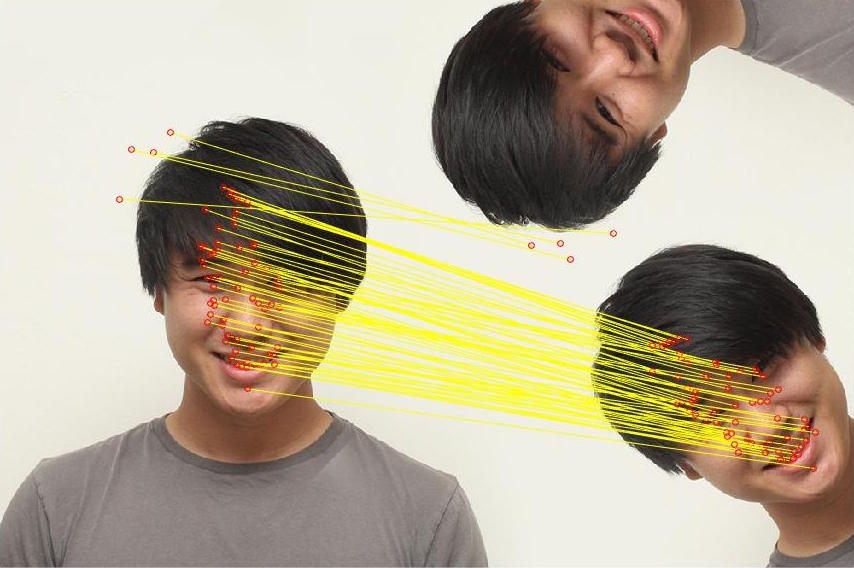
\includegraphics[width=.8\linewidth]{./gfx/with_rotation.jpg}
  \caption{With oriented box descriptors}
  \label{fig:sub2}
\end{subfigure}
\caption{The figure shows how copy-move detection is dramatically improved when orientation is taken into account for the descriptors.}
\label{fig:test}
\end{figure}

For SIFT, for each interest point, we take a 16x16 window around that point, splitting it into 4x4 windows. For each 4x4 window, we calculate the orientation and magnitude of the gradient at that point and bucket them into 8 buckets. We do this for each of the sixteen 4x4 windows for a total of 128 feature descriptors. Then, we subtract the magnitude and orientation of the interest point and normalize. To avoid any values that are significantly higher than the rest, we threshold the normalized vector at 0.2 and renormalize [?].

\subsection*{Matching}
After we have descriptors, we use the outlier rejection with nearest neighbor, heavily adapting the code from Efros et al.  Specifically, use a basic distance metric, Euclidean distance (our feature vector/descriptor is relatively low dimensional), to find the first and second nearest neighbor for each descriptor, and then we take the ratio of the distance. If that ratio is less than a threshold value, which we set to be 0.4, which the optimal value for panorama stitching [6]. In our experiments, we also tried to vary the threshold value. A smaller threshold value finds stronger matches, and subsequently makes running the estimated transformations faster. However, it can miss out on points. A large threshold will find more matches, but increases the running time of finding the set of estimated transformations. With our application, 0.4 was a good tradeoff between speed and breadth of points. A small detail worth mentioning is that for each descriptor point, we had to set the distance to itself to be infinity, otherwise it would find itself to be the nearest neighbor. 

To improve the speed of the subsequent step, we also do an additional step of filtering. We found that many points that were returned by the matching were points that were a few pixels away from each other, since the texture doesn't change too much. However, it is difficult by hand to copy move anything less than 10 pixels (or even 15-20 pixels). Therefore, we remove matches that are 3 pixels or less apart. 

\subsection*{Estimated Transformations}
Matching provides us with many correspondence points that have similar features, and we now use RANSAC to find the best set of matches that correspond to a copy move. RANSAC is an iterative method that repeatedly selects 4 points and computes the sum of squared differences (SSD) of each set of corresponding points [?]. Then, it keeps the set of inliers, where the SSD is less than some epsilon values. We run this for 8000 iterations. 

However, RANSAC has a single inlier set and therefore does not scale well to multiple translations. We derive a new method, multi-RANSAC (mRANSAC) that solves this issue. 

\section*{Results}

We benchmark our results on two metrics: number of points that were correctly matched, and time in seconds for completion. Additionally, we evaluate our results empirically and provide some examples that worked well and others that worked less well. Our numeric metrics are displayed in Table 1. 

\begin{table}[t]
\caption{Evaluation Metrics for Image: ?}
\label{image}
\begin{center}
\begin{tabular}{l|llllll}
\multicolumn{1}{l}{} & \multicolumn{1}{l}{\bf Box, ANMS} & \multicolumn{1}{l}{\bf Box, High} & \multicolumn{1}{l}{\bf BR, ANMS} & \multicolumn{1}{l}{\bf BR, High} & \multicolumn{1}{l}{\bf SIFT, ANMS} & \multicolumn{1}{l}{\bf SIFT, High}
\\ \hline \\
{\bf \# Points} & 0 & 0 & 0 & 0 & 0 & 0 \\
{\bf Time (s)} & 0 & 0 & 0 & 0 & 0 & 0 \\
\end{tabular}
\end{center}
\end{table}

\section*{Discussion and Future Work}

Discuss...

One area of future work include detecting scaled copy move detection. Currently SIFT is not sufficient for detecting copy move, and we propose a method to solve this problem: repeatedly downsize an image and run feature matching. However, this tends to be less common in copy move examples, as objects can appear out of place with too much scaling and are therefore more easily detected by the human eye. Another, albeit much more difficult, problem is to detect points that were warped with some homography. One potential solution to solving these problems is to instead form interest points in the frequency domain, a method that we hope will lead to uncover more underlying structure of an image and portions of the image. 

Another area of future work is to formalize mRANSAC and make it more robust to different images and arbitrary number clusters. We propose using some variant of the Hierarchical Dirichlet Process (HDP) to automatically find the clusters and be able to integrate it into the RANSAC algorithm. Our currently methodology is able to find points of the copy move, although it often just finds a portion of the copy move. The criterion of the inlier set could be experimented with in mRANSAC to be able to detect a wider spread of the copy move. 

Last, we propose two experiments for future work using our current framework to improve accuracy. The first is finding the optimal window size for each of the descriptors and developing a method of determining what window size to on which images. It is unclear whether using less points will increase or decrease the accuracy of the matching. Increase points will allow for more matches, but at the same time it will add more "noise". A formal assessment of this can determine the optimal number of points used. 

\subsection*{Acknowledgements}

We would like thank Alyosha Efros for teaching and inspiration, as well as the ideas from his panorama stitching project which greatly influenced our work. We thank James O'Brien for his initial guidance and support on this topic. We would additionally like to thank the University of Nurnberg for the dataset [2].

\subsection*{References}

\begin{enumerate}
\item B. Shivakumar et al. {\it Automated Forensic Method for Copy-Move Forgery Detection based on Harris Interest Points and SIFT Descriptors}. IJCA, August 2011. 
\item D. Lowe, {\it Distinctive image features from scale-invariant keypoints}. International Journal of Computer Vision, 60, 2 (2004), pp. 91-110.
\item {\it Image Manipulation Dataset}. http://www5.cs.fau.de/research/data/image-manipulation. 
\item J. Fridrich, D. Soukal and J. Lukas. {\it Detection of Copy-Move Forgery in Digital Images with}. Proc. of DFRWS 2003, Cleveland, OH, USA, August 5-8 2003
\item M. A. Fischler, R. C. Bolles. Random Sample Consensus: A Paradigm for Model Fitting with Applications to Image Analysis and Automated Cartography. Comm. of the ACM, Vol 24, pp 381-395, 1981. 
\item M. Brown and D. Lowe. {\it Automatic Panoramic Image Stitching using Invariant Features.} International Journal of Computer Vision. 74(1), pages 59-73, 2007.
\item M. Brown, R. Szeliski and S. Winder. {\it Multi-Image Matching using Multi-Scale Oriented Patches}. International Conference on Computer Vision and Pattern Recognition (CVPR2005) pp. 510-517.
\item S. Pittala. {\it Copy Move Forgery Detection using HOG Descriptor}.
\end{enumerate}

\subsection*{Appendix}

Image and stuff go here...

\end{document}

